\documentclass[
% twocolumn,
% hf, % comment this for submission
]{ceurart}

%%
%% One can fix some overfulls
\sloppy

%%
%% Minted listings support
%% Need pygment <http://pygments.org/> <http://pypi.python.org/pypi/Pygments>
\usepackage{listings}
\usepackage{todonotes}
\usepackage{import}
\usepackage{graphicx}
\usepackage{multirow}
\usepackage{graphicx}
\usepackage{float}
\usepackage[figuresleft]{rotating}

%% auto break lines
\lstset{breaklines=true}

%%
%% end of the preamble, start of the body of the document source.
\begin{document}
\appendix

\section{Appendix}
\label{sec:appendix}

\subsection{Results REBEL Model}
\begin{table}[!h]
	\centering
	\begin{tabular}{|l|l|l|l|l|l|l|}
		\hline
		\textbf{Relation} & \textbf{Precision} & \textbf{Recall} & \textbf{F1} & \textbf{Support} & \textbf{Micro F1}      & \textbf{Macro F1}      \\ \hline
		Cause             & 80.00              & 96.00           & 87.27       & 25               & \multirow{4}{*}{94.03} & \multirow{4}{*}{93.13} \\ \cline{1-5}
		Enable            & 94.55              & 94.55           & 94.55       & 55               &                        &                        \\ \cline{1-5}
		Prevent           & 98.21              & 91.67           & 94.83       & 60               &                        &                        \\ \cline{1-5}
		Intend            & 96.67              & 95.08           & 95.87       & 61               &                        &                        \\ \hline
	\end{tabular}
	\caption{Detailed result for the validation dataset using the REBEL model}
	\label{apx:val_result_rebel}
\end{table}

\begin{table}[!h]
	\centering
	\begin{tabular}{|l|l|l|l|l|c|l|}
		\hline
		\textbf{Relation} & \textbf{Precision} & \textbf{Recall} & \textbf{F1} & \textbf{Support} & \multicolumn{1}{l|}{\textbf{Micro F1}} & \textbf{Macro F1}      \\ \hline
		Cause             & 85.19              & 100.00          & 92.00       & 46               & \multirow{4}{*}{85.71}                 & \multirow{4}{*}{82.12} \\ \cline{1-5}
		Enable            & 84.62              & 61.11           & 70.97       & 18               &                                        &                        \\ \cline{1-5}
		Prevent           & 84.62              & 68.75           & 75.86       & 16               &                                        &                        \\ \cline{1-5}
		Intend            & 92.86              & 86.67           & 89.66       & 15               &                                        &                        \\ \hline
	\end{tabular}
	\caption{Detailed result for the test dataset using the REBEL model}
	\label{apx:test_result_rebel}
\end{table}

%Maybe break this images up, if it is not readable
\begin{figure}[!h]
	\centering
	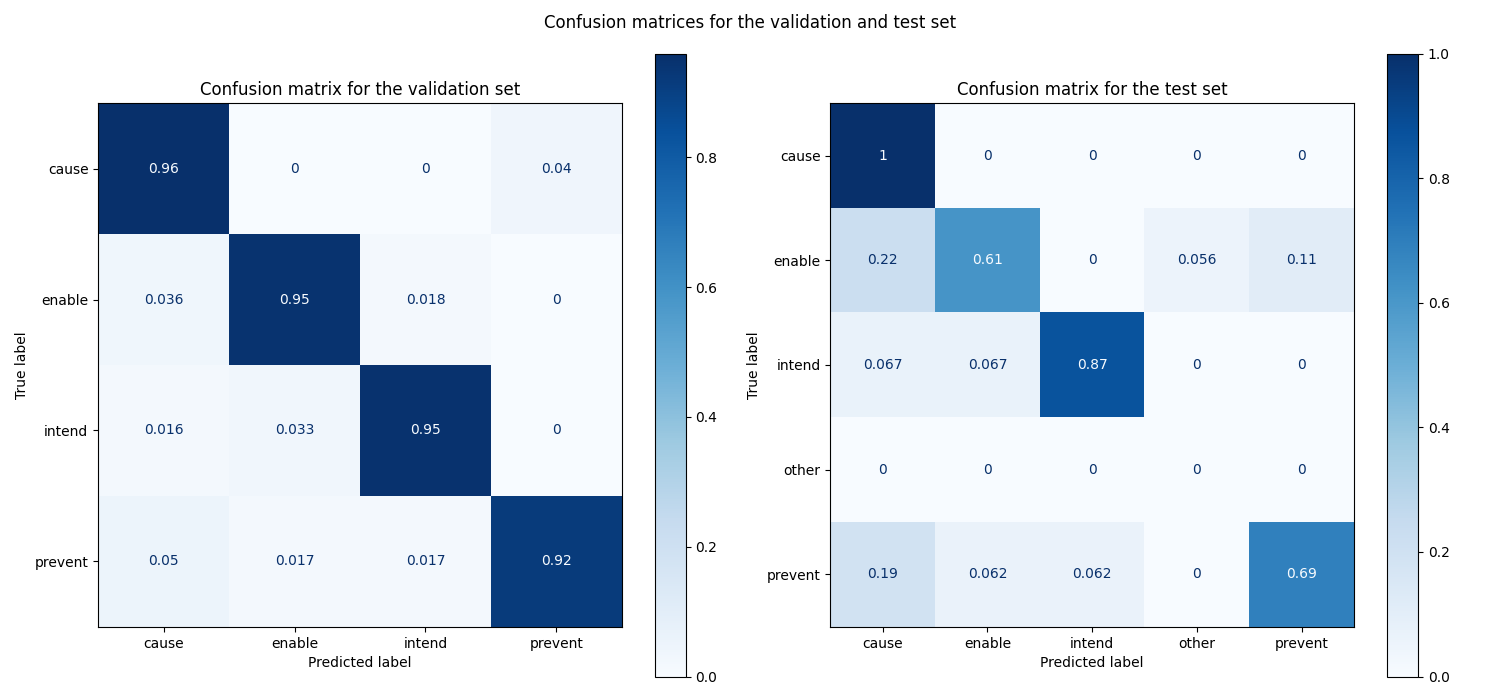
\includegraphics[width=1.2\textwidth]{Images/Confusion_matrix.png}
	\caption{Confusion matrix of relationships in the validation- and testset}
	\label{fig:confusion_matrix}
\end{figure}

\begin{table}[!h]
	\centering
	\begin{tabular}{|l|l|}
		\hline
		\textbf{Relation}    & \textbf{Frequency} \\ \hline
		has cause            & 1584               \\ \hline
		cause of destruction & 55                 \\ \hline
		has immediate cause  & 14                 \\ \hline
		immediate cause of   & 9                  \\ \hline
		end cause            & 3                  \\ \hline
		may prevent          & 2                  \\ \hline
	\end{tabular}
	\caption{Relationships in the REBEL train dataset}
	\label{apx:rebel_rel}
\end{table}

\subsection{Event coreference resolution}

\begin{figure}[!h]
	\centering
	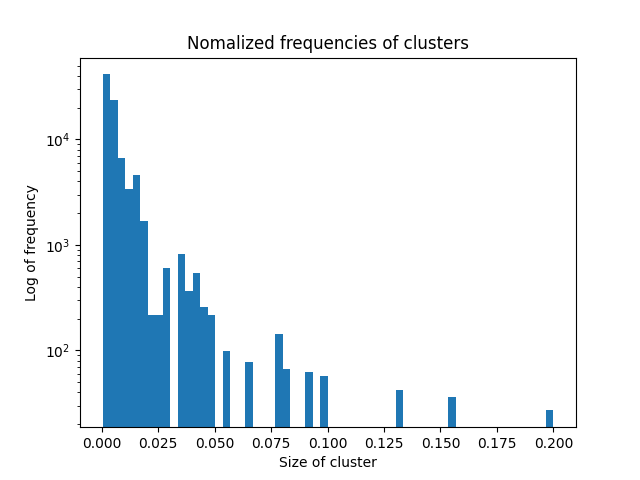
\includegraphics[scale=0.5]{Images/norm_freq_cluster_size.png}
	\caption{Normalized distribution of the cluster sizes}
	\label{fig:norm_freq_cluster_size}
\end{figure}

\subsection{JointGT: Qualitative analysis}
\begin{sidewaystable}[]
	\begin{tabular}{|l|l|l|}
		\hline
		\textbf{Triples}                                                                                                                                                                                                        & \textbf{Label}                                                                                                                                                                                                                                                                                                                                                                                                                                                                                       & \textbf{Generated}                                                                                                                                                                 \\ \hline
		\begin{tabular}[c]{@{}l@{}}(109 Felicitas, apoapsis, 523329000.0 (kilometres),\\ (109 Felicitas, temperature, 170.0 (kelvins))\end{tabular}                                                                             & \begin{tabular}[c]{@{}l@{}}(109 Felicitas , with a temperature of 170 kelvins , \\ has an apoapsis of 523329000.0 ( kilometres ) .), \\ (The temperature of the asteroid called 109 Felicitas is\\  170.0 kelvins and it has an apoapsis of 523329000.0 km .),\\ (The temperature of the asteroid called 109\\ Felicitas is 170.0 kelvins and it has an apoapsis of\\ 523329000 kilometres .)\end{tabular}                                                                                           & \begin{tabular}[c]{@{}l@{}}109 Felicitas has an apoapsis of 523329000.0\\ kilometres and a temperature of 170.0 kelvins .\end{tabular}                                             \\ \hline
		\begin{tabular}[c]{@{}l@{}}(3Arena, owner, Live Nation Entertainment),\\ (Dublin, is part of, Republic of Ireland),\\ (3Arena, location, Dublin),\\ (Dublin, is part of, Leinster)\end{tabular}                         & \begin{tabular}[c]{@{}l@{}}(The owner of 3Arena , Dublin , Leinster , \\ Republic of Ireland is Live Nation Entertainment .),\\ (Dublin is part of Leinster and a city in the Republic\\ of Ireland .Dublin is also home to the 3Arena which is\\ currently owned by Live Nation Entertainment .)\end{tabular}                                                                                                                                                                                       & \begin{tabular}[c]{@{}l@{}}3Arena is located in Dublin , Leinster , \\ Republic of Ireland and is owned by\\ Live Nation Entertainment .\end{tabular}                              \\ \hline
		(Barny Cakes, serving size, 30.0 g)                                                                                                                                                                                     & \begin{tabular}[c]{@{}l@{}}(Barny cakes can be served in 30 gram sizes .),\\ (Serving size for the Barny cakes is 30.0g .),\\ (The serving size of Barny cakes is 30.0g .)\end{tabular}                                                                                                                                                                                                                                                                                                              & Barny cakes have a serving size of 30.0 g .                                                                                                                                        \\ \hline
		\begin{tabular}[c]{@{}l@{}}(107 Camilla, discoverer, N.R. Pogson), \\ (N. R. Pogson, death place, Chennai),\\ (107 Camilla, periapsis, 479343000.0 (kilometres),\\ (N. R. Pogson, birth place, Nottingham)\end{tabular} & \begin{tabular}[c]{@{}l@{}}(Nottingham born , N.R . Pogson ( who died in Chennai ) ,\\ discovered 107 Camilla , which has a periapsis of\\ 479343000.0kilometres .), (N.R . Pogson discovered 107\\ Camilla which has a periapsis of 479,343,000 kilometres .\\ Pogson was born in Nottingham and died in Chennai .),\\ (107 Camilla was discovered by N.R . Pogson who was born\\ in Nottingham . He died in Chennai . The periapsis of 107\\ Camilla is 479343000.0 ( kilometres ) .)\end{tabular} & \begin{tabular}[c]{@{}l@{}}N.R . Pogson was born in Nottingham and\\ died in Chennai . He discovered 107 Camilla\\ which has a periapsis of479343000.0\\ kilometres .\end{tabular} \\ \hline
		('Fulton County, Georgia', country, United States)                                                                                                                                                                      & \begin{tabular}[c]{@{}l@{}}(Fulton County is in Georgia , in the United States .),\\ (Fulton County , in Georgia is part of the U.S .)\end{tabular}                                                                                                                                                                                                                                                                                                                                                  & Fulton County , Georgia is in the United States .                                                                                                                                  \\ \hline
	\end{tabular}
	\caption{Sample of the WebNLG testset and the generated output of the base model.}
	\label{tab:base_webnlgTestset}
\end{sidewaystable}


\clearpage
\begin{sidewaystable}[]
	\begin{tabular}{|l|l|l|}
		\hline
		\textbf{Triples}                & \textbf{Labels}                                                                                                                                                                                                                                                                  & \textbf{Generated}                        \\ \hline
		(demand, cause, benefited)      & \begin{tabular}[c]{@{}l@{}}(The company benefited from continued\\ strong demand and higher selling prices\\ for titanium dioxide, a white pigment used\\ in paints, paper and plastics.)\end{tabular}                                                                           & benefited '' is the cause of the demand . \\ \hline
		(center, enable, innovation)    & \begin{tabular}[c]{@{}l@{}}(We recently moved our headquarters and\\ research and development center to\\ Abu Dhabi to benefit from its rapidly\\ growing innovation hub, and with the new\\ AWS Region, we are excited to see it thrive\\ at an accelerated rate.)\end{tabular} & Innovation is the enabler of the center . \\ \hline
		(made, cause, eaten)            & \begin{tabular}[c]{@{}l@{}}("Cheerios and Honey Nut Cheerios have\\ eaten away sales normally going to Kellogg\'s\\ corn-based lines simply because they are\\ made of oats," says Merrill Lynch food\\ analyst William Maguire.)\end{tabular}                                   & The cause of eating is eaten .            \\ \hline
		(offer, cause, reimburse)       & \begin{tabular}[c]{@{}l@{}}(The directors said if Messrs. Drabinsky\\ and Gottlieb mail an offer to shareholders by\\ Nov. 22, it will reimburse them a maximum\\ of C\$8.5 million for expenses related to a bid.)\end{tabular}                                                 & The cause of the offer is to reimburse .  \\ \hline
		(proclaimed, prevent, bloodhed) & \begin{tabular}[c]{@{}l@{}}(DR Congo President Felix Tshisekedi on\\ May 6 proclaimed a 30-day "state of siege"\\ -- effectively martial law -- in North Kivu\\ and neighbouring Ituri province in a bid to\\ curb bloodshed by the ADF.)\end{tabular}                           & Bloodshed can be prevented .              \\ \hline
	\end{tabular}
	\caption{Sample of the FARO testset and the generated output of the base model}
	\label{tab:base_faroTestset}
\end{sidewaystable}


\clearpage
\begin{sidewaystable}[]
	\begin{tabular}{|l|l|l|}
		\hline
		\textbf{Triples}                & \textbf{Labels}                                                                                                                                                                                                                                                                  & \textbf{Generated}                                                                                                                                                                                            \\ \hline
		(demand, cause, benefited)      & \begin{tabular}[c]{@{}l@{}}(The company benefited from continued\\ strong demand and higher selling prices\\ for titanium dioxide, a white pigment used\\ in paints, paper and plastics.)\end{tabular}                                                                           & \begin{tabular}[c]{@{}l@{}}The company said it benefited from the strong demand\\ for its products and services from a growing number of customers.\end{tabular}                                              \\ \hline
		(center, enable, innovation)    & \begin{tabular}[c]{@{}l@{}}(We recently moved our headquarters and\\ research and development center to\\ Abu Dhabi to benefit from its rapidly\\ growing innovation hub, and with the new\\ AWS Region, we are excited to see it thrive\\ at an accelerated rate.)\end{tabular} & \begin{tabular}[c]{@{}l@{}}The United States has created a new innovation center that\\ will help stimulate economic growth and job creation.\end{tabular}                                                    \\ \hline
		(made, cause, eaten)            & \begin{tabular}[c]{@{}l@{}}("Cheerios and Honey Nut Cheerios have\\ eaten away sales normally going to Kellogg\'s\\ corn-based lines simply because they are\\ made of oats," says Merrill Lynch food\\ analyst William Maguire.)\end{tabular}                                   & \begin{tabular}[c]{@{}l@{}}The company said it made a profit from the sale of the shares\\ because it made enough money to make a profit from the sale.\end{tabular}                                          \\ \hline
		(offer, cause, reimburse)       & \begin{tabular}[c]{@{}l@{}}(The directors said if Messrs. Drabinsky\\ and Gottlieb mail an offer to shareholders by\\ Nov. 22, it will reimburse them a maximum\\ of C\$8.5 million for expenses related to a bid.)\end{tabular}                                                 & \begin{tabular}[c]{@{}l@{}}The company has also announced that it will offer a new credit\\ facility to small businesses, in an effort to reimburse them\\ for the cost of capital expenditures.\end{tabular} \\ \hline
		(proclaimed, prevent, bloodhed) & \begin{tabular}[c]{@{}l@{}}(DR Congo President Felix Tshisekedi on\\ May 6 proclaimed a 30-day "state of siege"\\ -- effectively martial law -- in North Kivu\\ and neighbouring Ituri province in a bid to\\ curb bloodshed by the ADF.)\end{tabular}                           & \begin{tabular}[c]{@{}l@{}}The United Nations has proclaimed a new resolution to\\ prevent the spread of bloodshed.\end{tabular}                                                                              \\ \hline
	\end{tabular}
	\caption{Sample of the FARO testset and the generated output of the combined model}
	\label{tab:combined_faroTestset}
\end{sidewaystable}
\clearpage

\subsection{Generating text from selected events}
\label{appx:selected_processed_events}

\textbf{Operation Breaking Dawn}
\begin{itemize}
	\item begin date: 2022-08-05
	\item end date: 2021-08-07
	\item location: Israel
	\item participant: Israel Defense Forces
	\item triples: $<bombardment,\;cause,\;firing>,\; <bombardment,\; cause,\; retaliated>,\; <fired,\; cause,\; killed>$
\end{itemize}
Base model: \textit{"Israel Defense Forces participated in Operation Breaking Dawn which began on August 5th, 2022 and ended on July 7th, 2022. The bombardment was retaliated by firing."}\\\\
\noindent
Combined model: \textit{"Israel Defense Forces participated in Operation Breaking Dawn which began on August 5th, 2022 and ended on July 7th, 2022. The Israelis were involved in Operation Breaking Dawn and were killed in the retaliation of the Israelis."}\\\\
\noindent

\textbf{2021 storming of the United States Capitol}
\begin{itemize}
	\item date: 2021-01-06
	\item location: United States of America
	\item participant: Proud Boys
	\item triples: $<measures,\;enable,\;removing>,\; <died,\; cause,\; shot>,\; <addressed,\; cause,\; shot>$
\end{itemize}
Base model: \textit{"Save America March is located in the United States of America and was launched on January 6th, 2021. Its cause was stormed and it was removed."}\\\\
\noindent
Combined model: \textit{"Save America March is located in the United States of America and was launched on January 6th, 2021. The US government has implemented a series of measures to prevent the spread of disasters."}\\\\
\noindent

\textbf{2021 Fukushima earthquake}
\begin{itemize}
	\item: date: 2021-02-13
	\item location: Japan
	\item triples: $<earthquake,\;cause,\;collapsing>,\; <earthquake,\; cause,\; injured>,\; <broken,\; cause,\; damage>$
\end{itemize}
Base model: \textit{"2021 Fukushima earthquake, which was caused by collapsing, is located in Japan and was broken."}\\\\
\noindent
Combined model: \textit{"The 2021 Fukushima earthquake, which hit Japan on February 13th, 2021, injured many people and caused extensive damage and collapsing."}\\\\
\noindent

\textbf{2021 Sundance Film Festival}
\begin{itemize}
	\item begin date: 2021-01-28
	\item end date: 2021-02-03
	\item location United States of America
	\item triples: $<whittled,\;cause,\;unveiling>,\; <awards,\; enable,\; stunt>,\; <coronavirus pandemic,\; cause,\; delayed>$
\end{itemize}
Base model: \textit{"2021 Sundance Film Festival, located in the United States of America, began on January 28th, 2021 and ended on March 3rd, 2021-02-03. The event was delayed by the coronavirus pandemic, and awards were whittled."}\\\\
\noindent
Combined model: \textit{"2021 Sundance Film Festival, which is located in the United States, began on January 28th, 2021 and ended on March 3rd, 2021. It was delayed because of the coronavirus pandemic."}\\\\
\noindent

\textbf{Giza church fire}
\begin{itemize}
	\item date: 2022-08-14
	\item location: Egypt
	\item triples: $<mobilized,\;cause,\;taken>,\; <went,\; cause,\; deaths>,\; <short circuit,\; cause,\; fire>$
\end{itemize}
Base model: \textit{"The cause of the Giza church fire, which was located in Egypt, was a short circuit. The church was mobilised on the 14th of August, 2022."}\\\\
\noindent
Combined model: \textit{"The Giza church fire, which occurred on 2022-08-14, was located in Egypt. It was a short circuit that killed several people."}\\\\
\noindent

\textbf{Nationwide COVID-19 memorial}
\begin{itemize}
	\item date: 2021-01-19
	\item location: United States of America
	\item triples: $<pandemic,\;prevent,\;swearing-in>,\; <confirmation,\; cause,\; run>,\; <sworn,\; cause,\; saluted>$
\end{itemize}
Base model: \textit{"The nationwide COVID-19 Memorial, located in the United States of America, was sworn in on January 19th, 2021. It was saluted and run to prevent a pandemic."}\\\\
\noindent
Combined model: \textit{"The National COVID-19 Memorial is located in the United States of America and was inaugurated
	on January 19th, 2021. It was saluted and sworn in to prevent a pandemic."}\\\\
\noindent

\textbf{Save America March}
\begin{itemize}
	\item date: 2021-01-06
	\item location: United States of America
	\item triples: $<measures,\;enable,\;removing>,\; <emergencies,\; cause,\; died>,\; <stormed,\; cause,\; drew>$
\end{itemize}
Base model: \textit{"Save America March is located in the United States of America and was launched on January 6th, 2021. Its cause was stormed and it was removed."}\\\\
\noindent
Combined model: \textit{"Save America March is located in the United States of America and was launched on January 6th, 2021. The US government has implemented a series of measures to prevent the spread of disasters."}



\subsection{Annotation of article: Russia launches Iranian satellite amid Ukraine war concerns}
\label{appx:article_annotation}

\textbf{An Iranian satellite launched by Russia blasted off from Kazakhstan Tuesday and reached orbit amid controversy that Moscow might use it to boost its surveillance of military targets in Ukraine}\\\\
\noindent
Triples: ("Russia", "launch", "satellite"), ("launch", "location", "Kazakhstan"), ("launch", "time", "Tuesday"), ("satellite", "enable", "military surveillance")\\\\
\noindent
Base model: \textit{"The launch of a satellite in Kazakhstan , which has a military surveillance capability , took place on Tuesday ."}\\\\
\noindent
Combined model: \textit{"The launch of a satellite from Russia was on Tuesday , in Kazakhstan . The satellite will enable military surveillance of the country ."}\\\\\\\\
\noindent
\textbf{As Russia's international isolation grows following Western sanctions over its invasion of Ukraine, the Kremlin is seeking to pivot towards the Middle East, Asia and Africa and find new clients for its embattled space programme.}\\\\
\noindent
Triples: ("Russia", "cause", "invasion of Ukraine"), ("invasion of Ukraine", "cause", "western sanctions"), ("western sanctions", "cause", "Russia's international isolation"), ("Russia", "intend", "find new clients")\\\\
\noindent
Base model: \textit{"Russia 's invasion of Ukraine is caused by western sanctions and Russia 's international isolation . Russia 's intention is to find new clients ."}\\\\
\noindent
Combined model: \textit{"The invasion of Ukraine is a cause of Russia 's isolation and western sanctions are a reason for Russia's invasion of Ukraine . Russia also seeks to find new clients in the region ."}\\\\\\
\noindent
\textbf{Speaking at the Moscow-controlled Baikonur Cosmodrome in the Kazakh steppe, Russian space chief Yury Borisov hailed "an important milestone in Russian-Iranian bilateral cooperation, opening the way to the implementation of new and even larger projects".}\\\\
\noindent
Triples: ("Russian-Iranian bilateral cooperation", "enable", "implementation of new and even larger projects")\\\\
\noindent
Base model: \textit{"The Russian-Iranian bilateral cooperation is enabled by the implementation of new and even larger projects ."}\\\\
\noindent
Combined model: \textit{"The Russian-Iranian bilateral cooperation will enable the implementation of new and even larger projects ."}\\\\\\
\noindent
\textbf{Iran's Telecommunications Minister Issa Zarepour, who also attended the launch of the Khayyam satellite, called the event "historic" and "a turning point for the start of a new interaction in the field of space between our two countries".}\\\\
\noindent
Triples: ("Iran Telecommunication", "minister", "Issa Zarepour"), ("Issa Zarepour", "attended", "launch of the Khayyam satellite"), ("satellite", "enable", "a turning point for the start of a new interaction")\\\\
\noindent
Base model: \textit{"Iran Telecommunications Minister Issa Zarepour attended the launch of the Khayyam satellite , which was a turning point for the start of a new interaction ."}\\\\
\noindent
Combined model: \textit{"Iran Telecommunication Minister Issa Zarepour attended the launch of the Khayyam satellite , which was a turning point for the start of a new interaction ."}\\\\\\
\noindent
\textbf{Nasser Kanani, the Iranian foreign ministry spokesman, said on Twitter that "the brilliant path of scientific and technological progress of the Islamic republic of Iran continues despite sanctions and the enemies' maximum pressure".}\\\\
\noindent
Triples: ("western sanctions", "not prevent", "scientific and technological progress of Iran"), ("enemies' maximum pressure", "not prevent", "scientific and technological progress of Iran")\\\\
\noindent
Base model: \textit{"The enemies ' maximum pressure is the scientific and technological progress of Iran ."}\\\\
\noindent
Combined model: \textit{"The United Nations has imposed a maximum pressure on Iran in an effort to prevent the country from achieving scientific and technological progress."}\\\\\\
\noindent
\textbf{Iran, which has maintained ties with Moscow and refrained from criticism of the Ukraine invasion, has sought to deflect suspicions that Moscow could use Khayyam to spy on Ukraine.}\\\\
\noindent
Triples: ("Iran", "maintained ties", "Moscow", 5), ("Iran", "not criticized", "Ukraine invasion", 5), ("Khayyam", "enable", "spy", 5)\\\\
\noindent
Base model: \textit{"Khayyam is a spy in Iran , which has maintained ties with Moscow . The Ukraine invasion is not criticized in Iran ."}\\\\
\noindent
Combined model: \textit{"Khayyam was allowed to spy on Moscow and Iran , which has not been criticized for its invasion of Ukraine ."}\\\\\\
\noindent
\textbf{Responding to the launch, Washington said Russia's growing cooperation with Iran should be viewed as a "profound threat".}\\\\
\noindent
Triples: ("Washington", "respond", "launch"), ("Russia's growing cooperation with Iran", "cause", "profound threat")\\\\
\noindent
Base model: \textit{"Russia 's growing cooperation with Iran is the cause of Washington 's response , which is a profound threat ."}\\\\
\noindent
Combined model: \textit{"Russia's growing cooperation with Iran has created a profound threat to the region, and the United States has responded with a missile launch."}\\\\\\
\noindent
\textbf{"No third country is able to access the information" sent by the satellite due to its "encrypted algorithm", it said.}\\\\
\noindent
Triples: ("satellite", "sends", "information"), ("encrypted algorithm", "prevent", "third countries accessing information"), ("satellite", "has", "encrypted algorithm")\\\\
\noindent
Base model: \textit{"The satellite has an encrypted algorithm which prevents third countries accessing information ."}\\\\
\noindent
Combined model: \textit{"The satellite sends information via an encrypted algorithm , which prevents third countries from accessing information ."}\\\\\\
\noindent
\textbf{Iran is currently negotiating with world powers, including Moscow, to salvage a 2015 deal aimed at reining in Tehran's nuclear ambitions.}\\\\
\noindent
Triples: ("Iran", "intend", "salvage 2015 deal"), ("2015 deal", "prevent", "Iran's nuclear ambitions")\\\\
\noindent
Base model: \textit{"Iran 's nuclear ambitions are intended to prevent the 2015 deal being salvaged ."}\\\\
\noindent
Combined model: \textit{"The United Nations has imposed a new nuclear deal on Iran in an effort to prevent the country from developing nuclear weapons."}\\\\\\
\noindent
\textbf{Western governments worry that satellite launch systems incorporate technologies interchangeable with those used in ballistic missiles capable of delivering a nuclear warhead, something Iran has always denied wanting to build.}\\\\
\noindent
Triples: ("satellite", "contains", "ballistic missle technologies", 9), ("ballistic missile technologies", "enable", "delivery of nuclear warhead", 9)\\\\
\noindent
Base model: \textit{"The satellite contains ballistic missile technologies which enable the delivery of nuclear warheads ."}\\\\
\noindent
Combined model: \textit{"The satellite contains ballistic missile technologies which enable the delivery of nuclear warheads ."}\\\\\\
\noindent
\textbf{Iran successfully put its first military satellite into orbit in April 2020, drawing a sharp rebuke from the United States.}\\\\
\noindent
Triples: ("Iran", "launch", "first military satellite", 10), ("first military satellite", "orbit", "April 2020", 10), ("first military satellite", "cause", "sharp rebuke from the United States", 10)\\\\
\noindent
Base model: \textit{"The first military satellite , launched in April 2020 , was launched in Iran . A sharp rebuke from the United States was the cause of the first military satellite ."}\\\\
\noindent
Combined model: \textit{"Iran launched its first military satellite in April 2020 , causing a sharp rebuke from the United States ."}\\\\\\
\noindent
\textbf{Borisov, who last month replaced bombastic nationalist Dmitry Rogozin as head of the Russian space agency, had acknowledged that the national space industry is in a "difficult situation" amid tensions with the West.}
\noindent
Triples: ("Borisov", "replaced", "Dmitry Rogozin", 11), ("Borisov", "acknowledged", "difficult situation", 11), ("tensions with the West", "cause", "difficult situation ", 11)\\\\
\noindent
Base model: \textit{"Borisov , who was replaced by Dmitry Rogozin , is in a difficult situation which has caused tensions with the West ."}\\\\
\noindent
Combined model: \textit{"Borisov , who was replaced by Dmitry Rogozin , acknowledged a difficult situation with the West because of tensions with the West ."}

\subsection{Example Narrative Graph of article: Russia launches Iranian satellite amid Ukraine war concerns}
\begin{sidewaysfigure}[hb]
	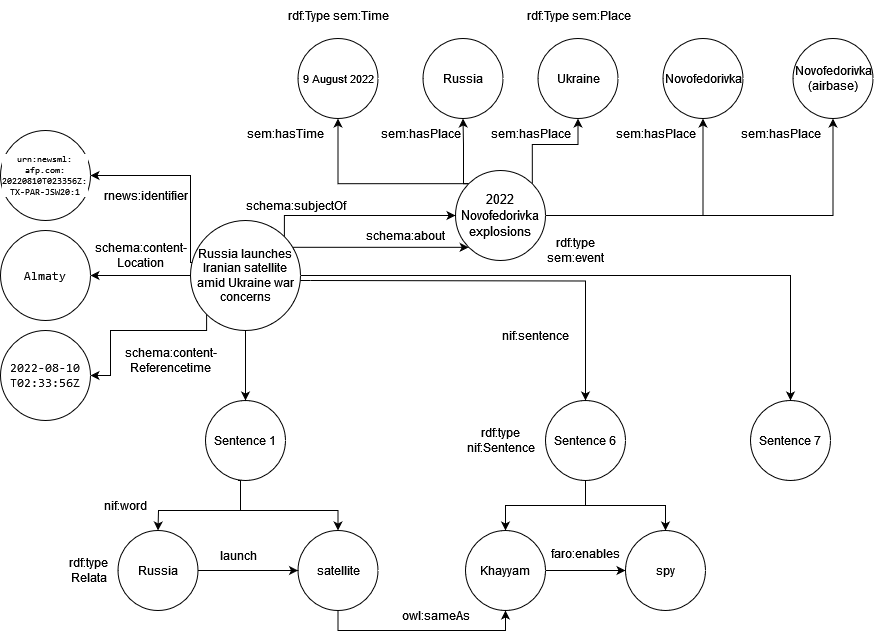
\includegraphics[scale=0.45]{Images/NG_article.png}
	\caption{Part of the constructed narrative graph of the article "Russia launches Iranian satellite amid Ukraine war concerns"}
	\label{fig:NG_article}
\end{sidewaysfigure}
\clearpage

\subsection{Overview Narrative Graph}
\begin{sidewaysfigure}[hb]
	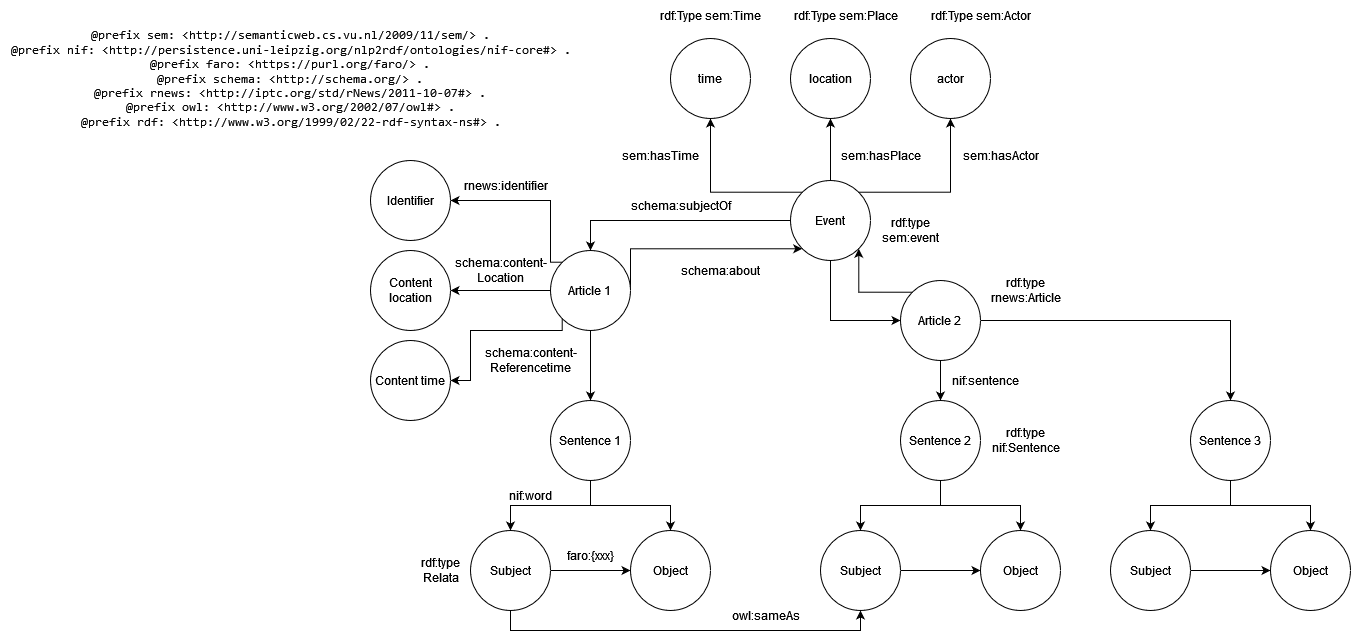
\includegraphics[scale=0.45]{Images/overview_graph.png}
	\caption{Overview of the Narrative Graph}
	\label{fig:graph_overview}
\end{sidewaysfigure}
% \clearpage


\end{document}